\documentclass{minimal}

\usepackage{tikz}
\usetikzlibrary{calc,positioning}

\newcommand{\drawstrangeborder}[1]{%
  \draw
    (#1.north west) --
    (#1.north east) --
    ($(#1.south east) + (0,.2)$) --
    ($(#1.south east) + (-.2,0)$) --
    ($(#1.south west) + (.2,0)$) --
    ($(#1.south west) + (0,.2)$) -- cycle;
}

\begin{document}
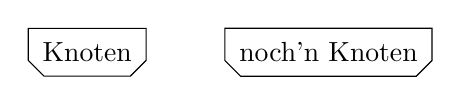
\begin{tikzpicture}
  \node[inner sep=5pt] (node) {Knoten};
  \drawstrangeborder{node};

  \node[inner sep=5pt, right=of node] (another node) {noch'n Knoten};
  \drawstrangeborder{another node};

\end{tikzpicture}
\end{document}